\chapter{Sistemi e Modelli}
In questa Capitolo vengono introdotti i concetti e una classificazione dei sistemi e
dei modelli ed il procedimento di creazione ed uso di un modello al fine di valutare le
prestazioni del sistema rappresentato.

\section{Definizione di sistemi e modelli}
Un sistema è rappresentato come un insieme di componenti (elementi, entità) interdipendenti e che interagiscono per raggiungere un determinato obiettivo. Un sistema di elaborazione è composto da componenti software, hardware e firmware che permettono l'elaborazione delle informazioni eseguendo programmi di utente.\\
Nello studio di un sistema devono essere considerati vari fattori fra cui:
\begin{itemize}
    \item funzionalità e correttezza;
    \item affidabilità;
    \item costo e fattori economici;
    \item prestazioni.
\end{itemize}
Le fasi di sviluppo e progettazione di un sistema sono:
\begin{itemize}
    \item \textbf{fase di progettazione:} in questa fase si sceglie il progetto del sistema fra diverse configurazioni disponibili;
    \item \textbf{fase di dimensionamento e acquisizione:} comprende la scelta fra diversi sistemi o componenti disponibili;
    \item \textbf{fase di evoluzione della configurazione e del carico:} si considerano tutti gli aspetti e i problemi relativi alla modifica ed evoluzione di un sistema esistente.
\end{itemize}
Le metodologie per la valutazione delle prestazioni di sistemi possono essere suddivise in due categorie:
\begin{itemize}
    \item tecniche di misurazione;
    \item tecniche modellistiche.
\end{itemize}
Le prestazioni possono essere quantificate tramite  di merito o indici di prestazioni che ne descrivono l'efficienza.
\begin{figure}[H]
	\centering
    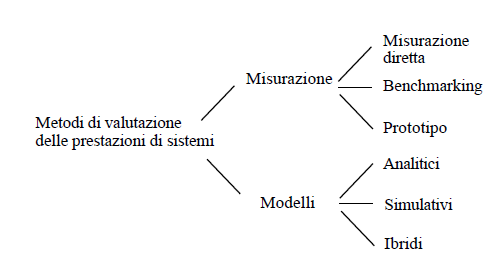
\includegraphics[width=15cm, keepaspectratio]{img/prestazioni.png}
	\caption{Metodi di valutazione delle prestazioni.}\label{fig:prestazioni}
\end{figure}
Come si può vedere in Figura \ref{fig:prestazioni} esistono diverse tecniche di misurazione:
\begin{itemize}
    \item \textbf{misurazione diretta}: il sistema vine misurato utilizzando il carico reale;
    \item \textbf{benchmark (carico artificiale)}: si ripete più volte il procedimento di misurazione e si effettuano misurazioni comparative fra diversi sistemi sotto le stesse condizioni di carico;
    \item \textbf{prototipazione}: se il sistema non è disponibile si può ricorrere alla costruzione di un prototipo su cui fare le misurazioni.
\end{itemize}


\paragraph{Definizione modello.}Un \textbf{modello} è una rappresentazione astratta del sistema che include solo gli aspetti rilevanti che servono per lo studio del sistema. Esso è definito da un certo livello di astrazione, cioè il sistema viene descritto con un certo livello di dettaglio riportando solo le componenti e le interazioni fra quest'ultimi necessari allo scopo prefissato.
\paragraph{Tecniche modellistiche.}
Si possono distinguere due tipologie di tecniche di modellazione:
\begin{itemize}
    \item \textbf{modello analitico}: variabili e parametri rappresentano le componenti e il carico del sistema, mentre le interazioni sono rappresentate tramite delle relazioni fra queste quantità;
    \item \textbf{modello di simulazione}: replica il comportamento dinamico di un sistema nel tempo rappresentando le componenti e le interazioni in termini di relazioni funzionali. La valutazione di quest'ultimo richiede l'esecuzione di un programma di simulazione o simulatore.
\end{itemize}

\paragraph{Vantaggi e svantaggi di un modello.}
I principali vantaggi nell'utilizzo di un modello per lo studio di un sistema sono:
\begin{enumerate}
    \item aumento e organizzazione delle conoscenze;
    \item analisi del sistema;
    \item modificabilità;
    \item diversi obbiettivi di studio.
\end{enumerate}
Invece gli svantaggi sono i seguenti:
\begin{enumerate}
    \item scelta del modello;
    \item uso errato del modello.
\end{enumerate}
 I modelli  che si basano su \textbf{processi stocastici} permettono di valutare la dinamica dei sistemi e in particolare le loro prestazioni e affidabilità. \\
 I \textbf{modelli a reti di code} permettono di rappresentare \textbf{sistemi di congestione}, i quali sono sistemi formati da un insieme limitato di risorse e in cui si osserva competizione per il loro utilizzo da parte di un insieme di utenti. Alcuni esempi di questi sistemi sono i sistemi di calcolo, di comunicazione. di traffico e di produzione. La valutazione delle prestazioni di un sistema di congestione include due differenti aspetti: dal punto di vista del sistema, si è interessati alla valutazione della utilizzazione delle risorse, mentre dal punto di vista dell’utente si valutano i tempi di attesa per l’uso delle risorse.
 
 \section{Classificazione di sistemi e di modelli}
 L'evoluzione nel tempo di un sistema è descritto dallo \textbf{stato} del sistema in ogni istante che ne rappresenta la condizione. Lo stato è espresso come \textbf{variabili di stato} che ne descrivono le entità e i loro attributi. Le attività delle componenti nel tempo e le interazioni fra queste sono descritte dalle \textbf{regole di trasformazione} fra stati. Il comportamento di un sistema nel tempo è rappresentato dalla \textbf{storia degli stati}. Le variabili di stato si distinguono in:
 \begin{itemize}
     \item \textbf{variabili endogene:} il loro cambiamento è dovuto soltanto ad attività interne al sistema. Il sistema si dice chiuso se il suo comportamento è determinato da queste variabili. 
     \item\textbf{ variabili esogene}: il loro cambiamento è influenzato dall'ambiente esterno al sistema. Il sistema si dice aperto se interagisce con l'ambiente esterno, utilizza anche variabili esogene. 
 \end{itemize}
 I sistemi possono essere suddivisi in \textbf{continui} e \textbf{discreti} a seconda del tipo di cambiamento dei valori delle variabili di stato, ad esempio se controlliamo la temperatura in un luogo la variabile che la rappresenta è continua poiché verifichiamo i cambiamenti nel tempo.\\
 Il modo in cui avvengono le trasformazioni fra stati determina se un sistema è \textbf{deterministico} o \textbf{stocastico}, nel primo caso le regole di trasformazione determinano il cambiamento del sistema in modo univoco mentre nel secondo si può passare da uno stato a un altro secondo diverse leggi/distribuzioni di probabilità. La natura del sistema dipende anche dalla visione dell'osservatore che è definita dagli obiettivi e dal metodo di studio. A loro volta anche i modelli possono essere distinti in queste categorie con la differenza che un modello associato un sistema non deve necessariamente corrispondergli, esempio un sistema deterministico definito da un modello stocastico. \\
 I modelli si distinguono in due principali categorie:
 \begin{itemize}
     \item modelli fisici;
     \item modelli simbolici: questi includono i modelli matematici e non.
 \end{itemize}
 
 
 
\section{Ciclo dei modelli}
Il procedimento di creazione di un modello è un processo iterativo di raffinamenti successivi, vengono fatte delle assunzioni ed ipotesi da verificare e valutare.
Il processo di creazione ed uso di un modello può essere schematizzato come segue:
\begin{enumerate}
    \item \textbf{Definizione degli obiettivi:} definizione e comprensione del sistema oggetto di studio e delle sue componenti. Si stabiliscono anche i criteri di valutazione delle soluzioni e si acquisiscono i dati dal sistema misurandone anche il carico.
    \item \textbf{Definizione del modello e formulazione delle assunzioni e ipotesi:} vengono identificate le componenti del modello così come le assunzioni ed ipotesi utilizzate.
    \item \textbf{Parametrizzazione:} sono identificate le variabili del modello da misurare e gli strumenti di misurazione.
    \item \textbf{Valutazione (soluzione) del modello e interpretazione dei risultati:} definito e parametrizzato il modello si sceglie il metodo di soluzione più appropriato.
    \item \textbf{Validazione del modello e valutazione dei risultati:} si valuta il modello nella descrizione del sistema se questo risulta non soddisfacente si itera ai passi 1, per ridefinire il sistema e gli obiettivi, o 2, per modificare la definizione del modello e delle ipotesi, o 3, per ri-parametrizzare le variabili.
    \item \textbf{Documentazione e analisi della sensitività:} riporta i risultati trovati compresi i dettagli relativi al modello e anche una descrizione del processo di definizione del modello.
\end{enumerate}

\begin{figure}[H]
	\centering
    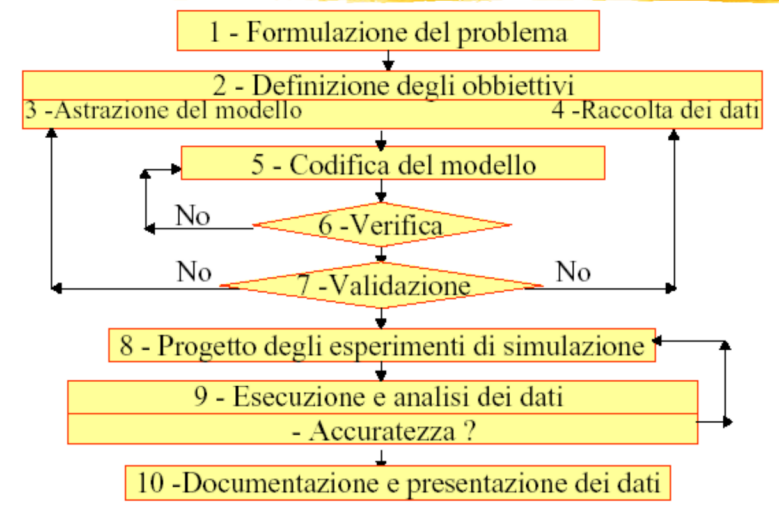
\includegraphics[width=15cm, keepaspectratio]{img/ciclo_modello.png}
	\caption{Ciclo di vita di un modello.}\label{fig:ciclo_modello}
\end{figure}

\section{Schemi di simulazione}
Sono delle strutture di modelli di simulazione che differiscono in base ai tre concetti di evento, attività e processo. Ne esistono quattro metodologie:
\begin{itemize}
    \item Interazione fra processi
    \item Scheduling di eventi
    \item Scansione di attività
    \item Metodo a Tre fasi
\end{itemize}

\subsection{Schemi di simulazione: processi}
Il flusso di esecuzione di un processo permette di simulare il comportamento di un oggetto (entità) attraverso il sistema. L'esecuzione del processo continua fintanto che non viene bloccato, sospeso o arriva un'altra entità. Nel caso in cui il flusso viene bloccato, si avanza nel tempo fino ad arrivare al punto di inizio dell'esecuzione della prossima attività.
\paragraph{Esempio: scheduling dei processi}
In un sistema di elaborazione ogni processo viene eseguito ciclicamente supponiamo che si utilizzi la disciplina FIFO per gestire la coda di processi, i passi eseguiti sono i seguenti:
\begin{enumerate}
    \item Esamina la coda, se vuota vai a 5
    \item Preleva un job dalla coda
    \item Esegui il servizio per il job
    \item Vai al passo 1
    \item Attendi l'arrivo del prossimo utente, quando arriva vai al passo 1
\end{enumerate}
Il punto 4 è un punto di sospensione o si riattivazione del processo, al contrario nel passo 5 il processo è in stato passivo fino a che non arriva un job. In generale nella simulazione fra processi esiste una routine che gestisce i cambiamenti di stato dei processi, essa controlla due code diverse:
\begin{itemize}
    \item \textbf{processi bloccati}: contiene gli oggetti sospesi
    \item \textbf{processi sospesi}: contiene gli oggetti passivi
\end{itemize}
La routine permette di riattivare un oggetto, il quale può essere:
\begin{itemize}
    \item \textbf{attivo:} esegue azioni
    \item \textbf{sospeso:} ha un tempo di riattivazione
    \item \textbf{passivo:} non è attivo e il tempo di riattivazione dipende da un altro oggetto
    \item \textbf{terminato:} ha terminato il suo lavoro
\end{itemize}

\subsection{Schemi di simulazione: eventi}
Nella simulazione per scheduling di eventi si avanza il tempo simulato al tempo del prossimo evento che coincide spesso con il termine di un'attività o l'inizio. In questo caso gestiamo una lista ordinata di eventi e scheduler di eventi. Lo scheduler di eventi gestisce il tempo simulato mantenendo una lista ordinata di eventi futuri:
\begin{itemize}
    \item \textbf{event-driven}: clock= tempo del prossimo evento in lista
    \item \textbf{unit-time:} $clock= clock + \Delta$
\end{itemize}
Inoltre esso gestisce anche la struttura dati che contiene tutti gli eventi e anche la routine evento.
Quest'ultima permette di aggiornare sia la lista di variabili di stato che la lista di eventi, essa può essere di:
\begin{itemize}
    \item \textbf{inizializzazione}:chiamata per prima e definisce le variabili di stato ed altro;
    \item \textbf{gestione degli eventi};
    \item \textbf{ trace}: serve per notificare eventi o stime a run-time;
\end{itemize}


\subsection{Schemi di simulazione: attività}
La simulazione avviene scansionando le attività ovvero descrivendone le componenti del modello. Se è applicato il meccanismo di avanzamento per intervalli fissi $\Delta$, ad ogni avanzamento vengono esaminate tutte le attività per stabilire le condizioni di inizio e di fine. Le procedure aggiornano lo stato della singola attività. Si può anche applicare un meccanismo di avanzamento del tempo distribuito nelle procedure delle attività simile all'avanzamento per eventi.

\subsection{Schemi di simulazione: "tre fasi"}
Nella simulazione a "tre fasi" si ha un avanzamento del tempo per intervalli fissi, le varie fasi che la compongono sono:
\begin{itemize}
    \item  fase 1: avanzamento del tempo simulato;
    \item fase 2: rilascio risorse mantenute dalle attività che risultano terminate dopo l'avanzamento;
    \item fase 3: esecuzione delle attività per la quali siano ora disponibili le risorse.
\end{itemize}

